\documentclass{article}
\usepackage{subcaption}


% Language setting
% Replace `enapplicationglish' with e.g. `spanish' to change the document language
\usepackage[english]{babel}

% Set page size and margins
% Replace `letterpaper' with `a4paper' for UK/EU standard size
\usepackage[letterpaper,top=2cm,bottom=2cm,left=3cm,right=3cm,marginparwidth=1.75cm]{geometry}

% Useful packages
\usepackage{amsmath}
\usepackage{graphicx}
\usepackage[colorlinks=true, allcolors=blue]{hyperref}

\title{MoSIS Assignment 1: Modelica}
\author{Stein Vandenbroeke s0205627 & Niels Van den Broeck s0203844}

\begin{document}
\maketitle

\section{Plant Model Creation}

In the first part of the assignment, we made the gantry system using textual equations in Modelica. After converting the variables, parameters and equations from the assignment into Modelica, we ended up with the following code:

\begin{verbatim}
model Gantry_system
  // Variables
  Modelica.Units.SI.Length x "displacement of the trolley/cart expressed in m";
  Modelica.Units.SI.Velocity v "velocity of the trolley/cart expressed in m/s";
  Modelica.Units.SI.Angle theta "Angular displacement of the pendulum w.r.t 
    the trolley expressed in rad";
  Modelica.Units.SI.AngularVelocity w "Angular velocity of the pendulum expressed in rad/s";
  Real u "Control signal to move the trolley and pendulum";
  
  // Parameters
  parameter Modelica.Units.SI.Mass m = 0.2 "Mass of pendulum bob/container expressed in kg";
  parameter Modelica.Units.SI.Mass M = 10 "Mass of trolley/cart expressed in kg";
  parameter Modelica.Units.SI.Length r = 1 "Length of the rope connecting the pendulum bob
    to the trolley expressed in m";
  parameter Modelica.Units.SI.Damping dp = 0.5 "Damping factor swinging of pendulum
    expressed in s-1";
  parameter Modelica.Units.SI.Damping dc = 2 "Damping factor for motion of cart
    expressed in m/s^2";
  parameter Modelica.Units.SI.Acceleration g = Modelica.Constants.g_n;
  
  // Initial values for the variables
initial equation
  x = 0;
  v = 0;
  theta = 0;
  w = 0;
  
equation  
  if time < 0.5 then
   u = 1000;
  else 
   u = 0;
  end if;
  der(x) = v;
  der(theta) = w;
  der(v) = (r*(dc*v - m*(g*sin(theta)*cos(theta) + r*sin(theta)*w^2) - u) - 
    (dp*cos(theta)*w))/(-r*(M + m*(sin(theta))^2));
  der(w) = ((dp*w*(m + M)) + (m^2*r^2*sin(theta)*cos(theta)*w^2) + 
    m*r*((g*sin(theta)*(m + M)) + (cos(theta)*(u - dc*v))))/((m*r^2)*(-M - (m*sin(theta)^2)));
end Gantry_system;
\end{verbatim}

\begin{figure}[h]
    \begin{subfigure}[b]{0.5\textwidth}
        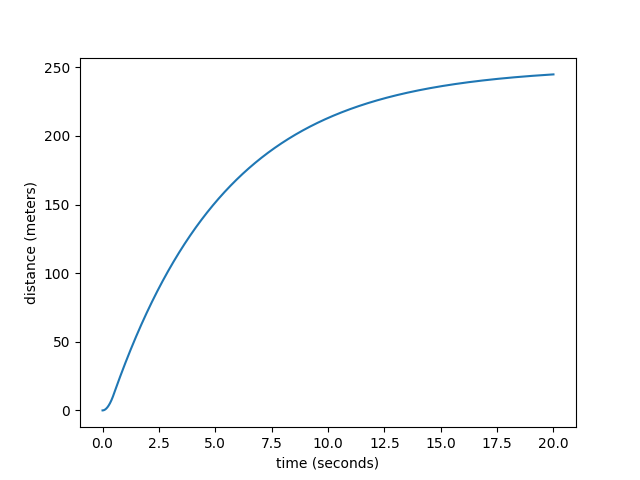
\includegraphics[width=\linewidth]{graphs/gantry_system_displacement.png}
        \caption{Displacement}
    \end{subfigure}
    \begin{subfigure}[b]{0.5\textwidth}
        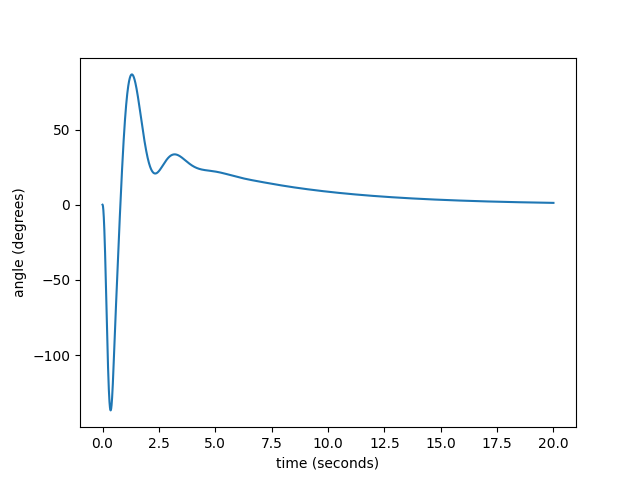
\includegraphics[width=\linewidth]{graphs/gantry_system_angular_displacement.png}
        \caption{Angular displacement}
    \end{subfigure}
    \caption{Plots}
    \label{fig:gantry_system}
\end{figure}

Simulating this model for 20 seconds with a step size of 0.004 seconds resulted in the graphs shown in Figure \ref{fig:gantry_system}. 

During the initial 0.5 seconds of the simulation, the control signal to move the trolley is set to 1000, which results in an increasing velocity and thus movement of the trolley. this is visible in the first graph where the displacement starts from 0 and exponentially rises until approximately 0.5 seconds. Due to Newton's Second Law (F = ma), when the trolley moves to the right, an inertial force acts on the pendulum, causing it to stay behind. This creates a negative angle between the pendulum and the trolley. After some time, the influence of gravity becomes apparent and and the pendulum begins to swing, making the angle go up and down. 

After these 0.5 seconds, the control signal is set to zero, which causes the trolley and pendulum to slowly decelerate. 

Note. due to the pull exerted from the trolley, along with the influence of gravity, We anticipated the pendulum to have a slight negative angle after a few seconds, when the swinging fades out. However, after running the animation, we saw that this was not the case and instead of a negative angle, it got a positive angle. A review of the graph confirmed this observation. After roughly 5 seconds, the pendulum stops swinging i.e. the angle function does not alternate between a positive slope and a negative slope. This seemed to be a flaw in our model, but after careful inspection, we found that the reason for this behavior is the deceleration of the trolley. In this period, the momentum of the pendulum from the acceleration is still present and thus it wants to lean to the right.

\section{Plant Model Calibration}

\begin{figure}[h]
    \begin{subfigure}[b]{0.5\textwidth}
        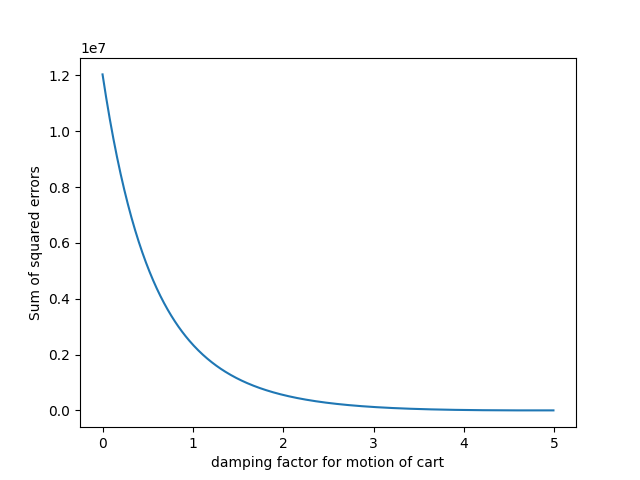
\includegraphics[width=\linewidth]{graphs/dc_calibration.png}
        \caption{Errors of different damping factors}
    \end{subfigure}
    \begin{subfigure}[b]{0.5\textwidth}
        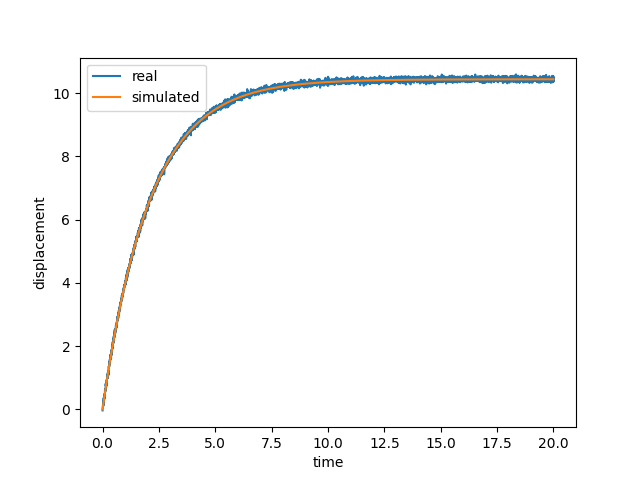
\includegraphics[width=\linewidth]{graphs/dc_displacement_error.png}
        \caption{Simulated displacement vs real displacement}
    \end{subfigure}
    \caption{Damping factor for the motion of the cart}
    \label{fig:dc}
\end{figure}

\subsection{Damping factor for the motion of the trolley/cart}

To find the optimal damping factor for the motion of the trolley: dc, a python script is created to test every possible value between 0 and 5, with a precision of 2 decimals. The code can be found in \textit{parameter\_tuning.py}. For each dc, the sum of squared errors between the simulation and the given real-life data is calculated. When the error is large, the damping factor deviates from reality, while a small error concludes in a simulation that is close to reality. We found that the optimal value of this damping factor is 4.79. In Figure \ref{fig:dc}, graph (a) shows the different tested values of dc and their corresponding error from real life data. In graph (b), the displacement of the trolley is shown over time for the real data (in blue) and the simulation with the corresponding dc = 4.79 (in orange). The values clearly show a strong alignment.

\begin{figure}[h]
    \begin{subfigure}[b]{0.5\textwidth}
        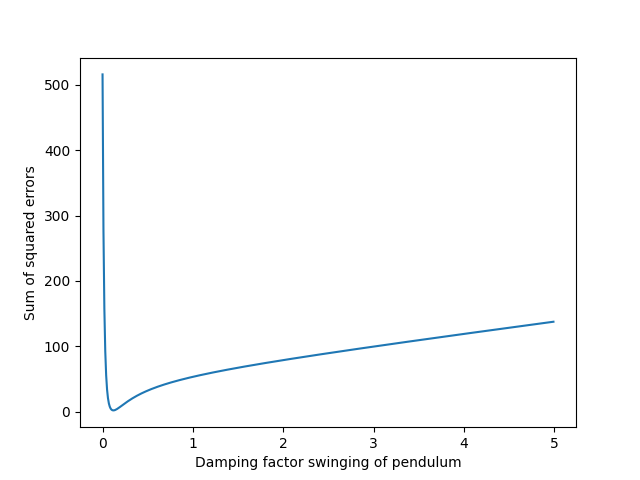
\includegraphics[width=\linewidth]{graphs/dp_calibration.png}
        \caption{Errors of different damping factors}
    \end{subfigure}
    \begin{subfigure}[b]{0.5\textwidth}
        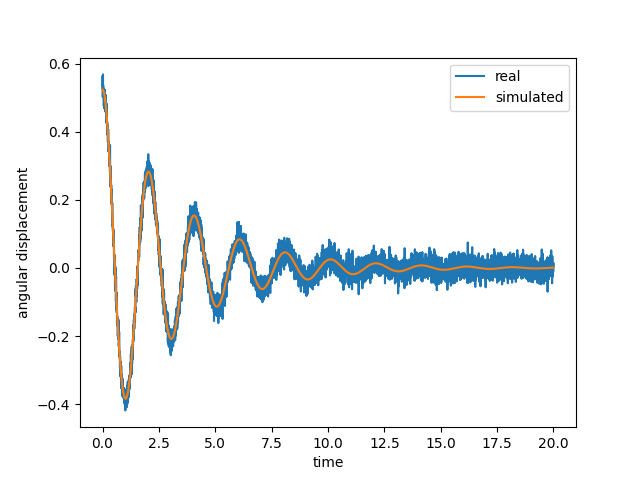
\includegraphics[width=\linewidth]{graphs/dp_displacement_error.png}
        \caption{Simulated displacement vs real displacement}
    \end{subfigure}
    \caption{Damping factor for the swinging of the pendulum}
    \label{fig:dp}
\end{figure}

\subsection{Damping factor for the swinging of the pendulum}

In the same python file, you can find the code to calibrate the damping factor for the swinging of the pendulum: dp. The same principle is applied as for dc, but now for the angular displacement of the pendulum. In Figure \ref{fig:dp}, graph (a) shows that dp should be around 0.1 for the smallest possible error. Running the python script confirmed this and gave 0.12 as the optimal value of dp. In graph (b), the angular displacement of the pendulum is shown over time for the real data (in blue) and the simulation with the corresponding dp = 0.12 (in orange). These plots are, once again, largely the same.

\section{Controller Model Creation}

\begin{figure}[h]
    \begin{subfigure}[b]{0.5\textwidth}
        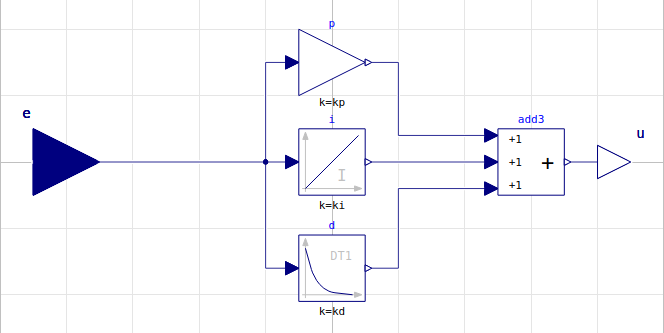
\includegraphics[width=\linewidth]{graphs/PID_block.png}
        \caption{PID block}
    \end{subfigure}
    \begin{subfigure}[b]{0.5\textwidth}
        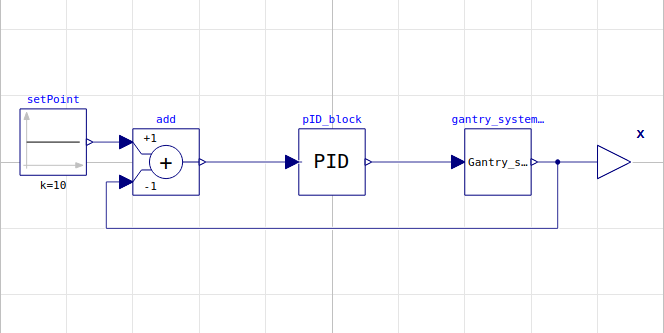
\includegraphics[width=\linewidth]{graphs/PID_controller_block.png}
        \caption{PID controller block}
    \end{subfigure}
    \caption{Controller Model}
    \label{fig:PID}
\end{figure}

\subsection{Kp-value}
\begin{figure}[h]
    \centering
    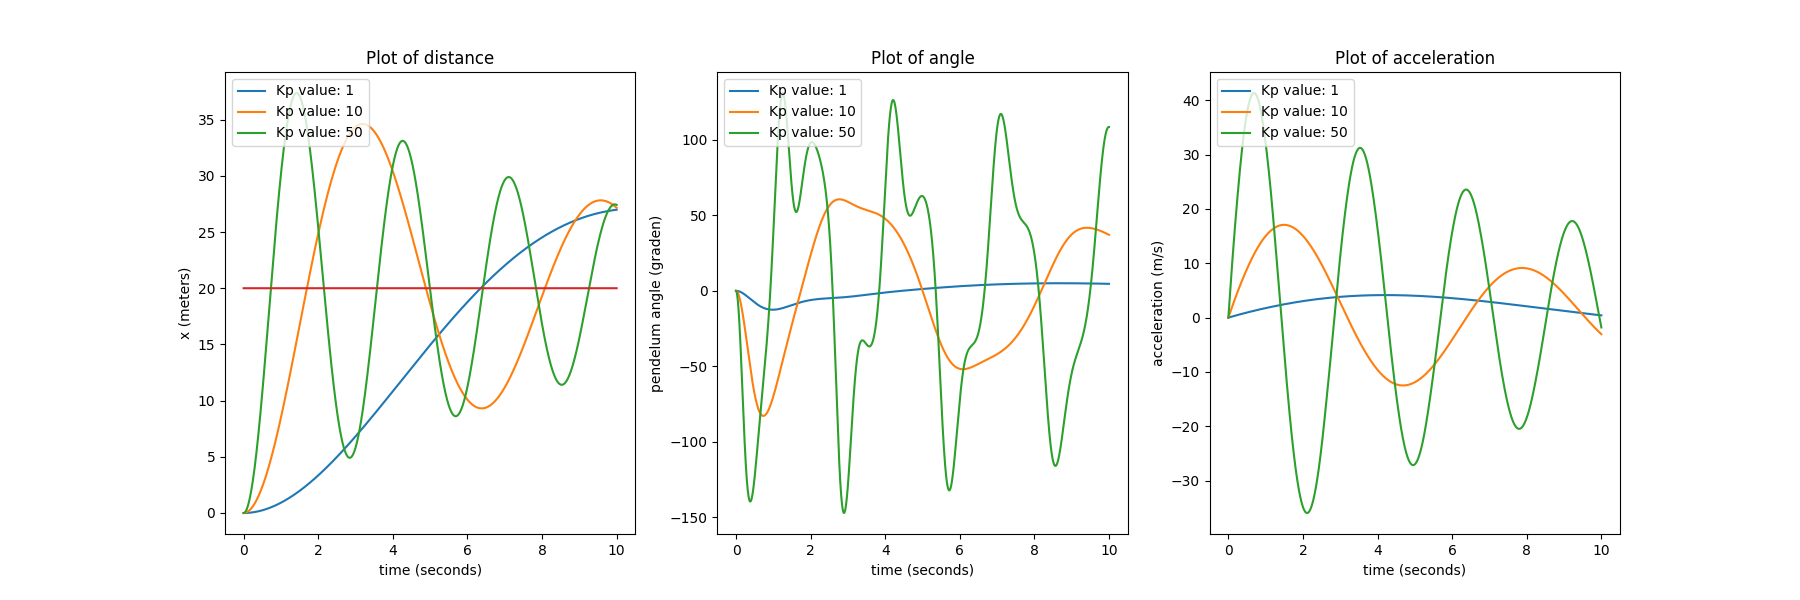
\includegraphics[width=1\linewidth]{graphs/kp_test.png}
    \caption{Kp value test for Kp = 1, 10, 50}
    \label{fig:kp-test}
\end{figure}
The Kp value corresponds to the constant gain multiplied by the error. In our case this value impacts how fast the trolley accelerates and decelerates depending on how much error there is with respect to the set-point.
This is visible in Figure \ref{fig:kp-test}, Where a higher Kp value leads to a higher velocity in a shorter time, and thus the set-point is approached rather quickly, but there is a lot of overshoot.

\subsection{Ki-value}
\begin{figure}[h]
    \centering
    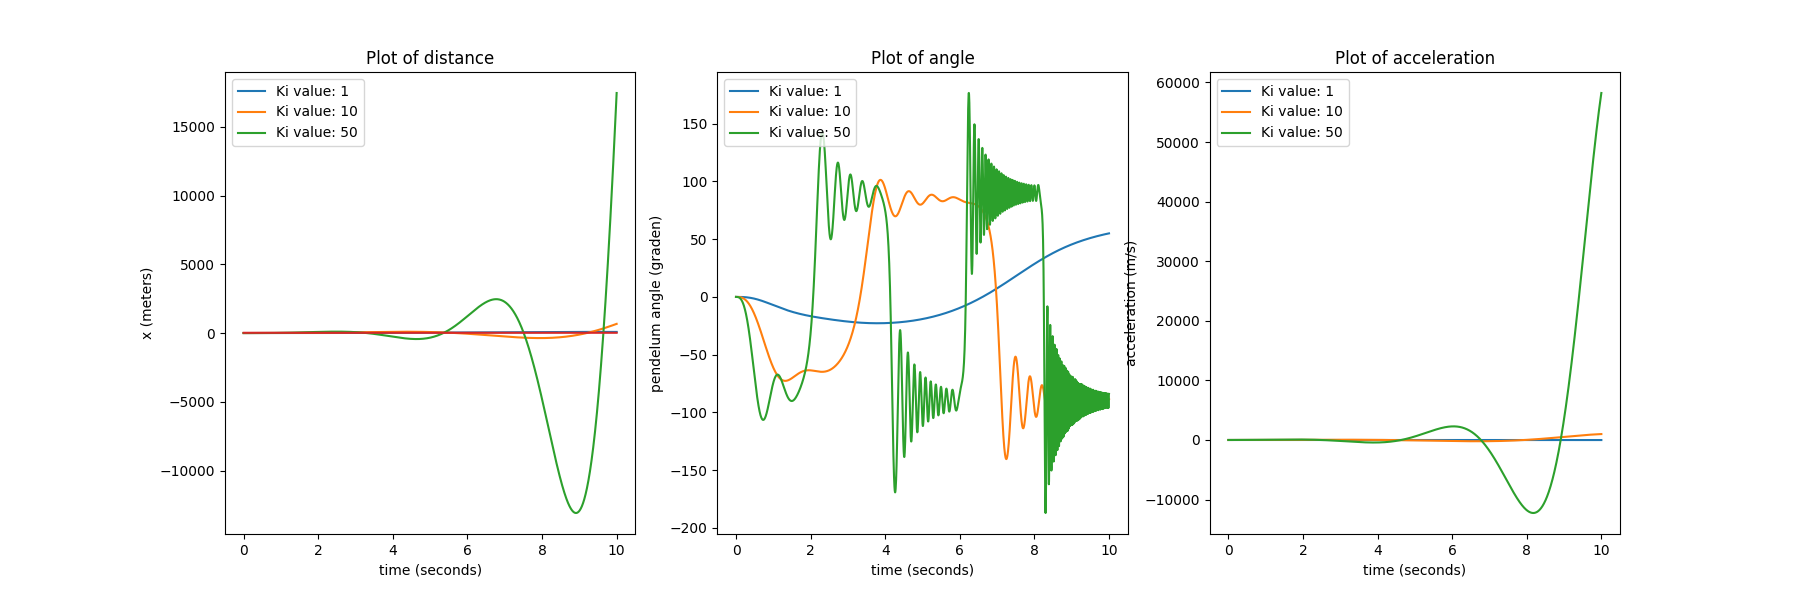
\includegraphics[width=1\linewidth]{graphs/ki_test.png}
    \caption{Ki value test for Ki = 1, 10, 50}
    \label{fig:ki-test}
\end{figure}

The Ki value is the constant gain for the integral of the error over time. This results in the PID trying to get an average result value that is the same as the set-point,
and thus in our case a useless parameter that should be set to 0. This is the case because we do not want our distance to average above the set-point (We must reach the point as quickly as possible and then stay still). In Figure \ref{fig:ki-test}, we see that the function will first overshoot the set-point to compensate for the start at 0. Because of the momentum of the trolley, this effect will spiral out of control quickly.

\subsection{Kd-value}
The Kd value is the the constant gain for the derivative of the error over time. This will result in a large compensation value when the error is big, but will quickly adjust as the error get smaller. In terms of the trolley movement this means that we have a large spike in acceleration followed by a quick deceleration. This results in large amount of rotations of the pendulum. See Figure \ref{fig:kd-test}.
\begin{figure}[h]
    \centering
    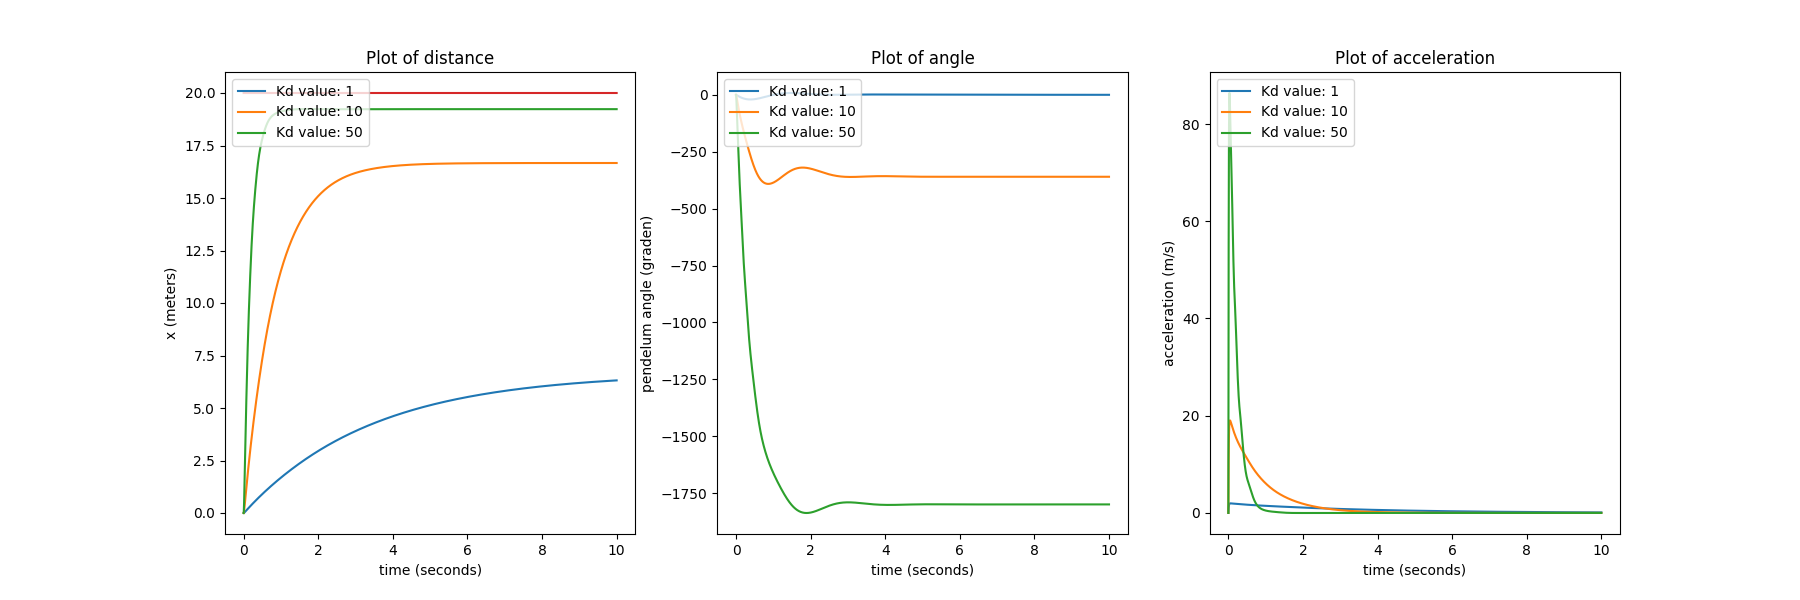
\includegraphics[width=1\linewidth]{graphs/kd_test.png}
    \caption{Kd value test for Kd = 1, 10, 50}
    \label{fig:kd-test}
\end{figure}
<
\section{Controller Model Tuning}

\begin{figure}[h]
    \begin{subfigure}[b]{0.5\textwidth}
        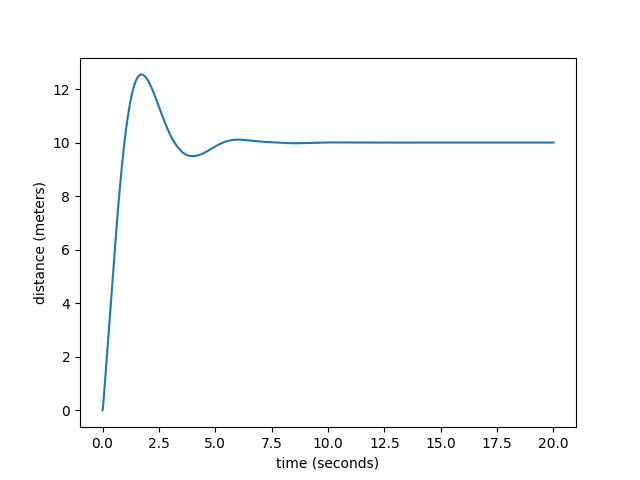
\includegraphics[width=\linewidth]{graphs/PID_optimal_distance.png}
        \caption{PID optimal distance}
    \end{subfigure}
    \begin{subfigure}[b]{0.5\textwidth}
        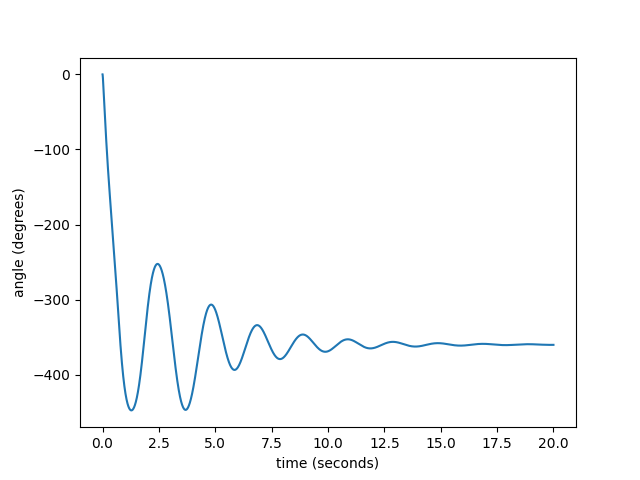
\includegraphics[width=\linewidth]{graphs/PID_optimal_theta.png}
        \caption{PID optimal angle}
    \end{subfigure}
    \caption{optimal PID controller simulation}
    \label{fig:optimal_PID}
\end{figure}

Our personal cost function for this subtask is:
\begin{equation} cost = 94 \cdot \theta_{max} + 71 \cdot t_{task} \end{equation}
where we changed a with 94 and b with 71 according to the 'group-specific cost-function parameters'.

To find the best possible parameter values for $K_p ([1,40])$ and $K_d ([10,500])$, another script is made which can be found in \textit{parameter\_tuning.py}. We had to increase the simulation time to 100 seconds since some of the simulations did not get to the final position with corresponding angle in time. We found that the best values for $K_p$ and $K_d$ are 26 and 10 respectively. When we simulate the PID controller for the gantry system with the optimal control parameters, we get the graphs shown in Figure \ref{fig:optimal_PID}. Graph (a) shows the distance that the trolley travels over the rack. You can see that it first overshoots until around 12 meters and then comes back to stable out at 10 meters. When we look at the second graph (b), we see that the angle quickly goes to -400 degrees, which indicates that the pendulum made a whole loop. After that it gets balanced to -360 degrees. This is the same as 0 degrees and thus the requirements are reached at around 9 seconds. This unexpected movement of a complete rotation is the result of the cost function not punishing enough for the max angle. In real life, this would not be ideal, since we do not want a container with a high weight to spin around like that. A possible explanation to this is that we set the trolley and the pendulum's weight to only 10 and 0.2 kg respectively. To solve this issue, we could create another cost function which takes these requirements into account, or use more realistic values for the trolley and pendulum.

\bibliographystyle{alpha}
\bibliography{sample}

\end{document}